\documentclass[aspectratio=169]{beamer}

\usepackage[utf8]{inputenc}
\usepackage{graphicx}
\usepackage{tikz}
\usetikzlibrary{positioning, arrows.meta}

\usefonttheme{professionalfonts}

% Theme — RSP format
\usetheme{Madrid}
\definecolor{ucdgreen}{RGB}{0, 102, 51}
\definecolor{lightblue}{RGB}{100, 160, 210}
\usecolortheme[named=lightblue]{structure}
\setbeamertemplate{navigation symbols}{}
\setbeamersize{text margin left=10mm, text margin right=4mm}

\title[Earth Day Flash Talk]{}
\author[Lainey Ward]{}
\institute[]{}
\date{}

\begin{document}

\begin{frame}{Navigating the Predictability Desert}

    \begin{columns}[c, totalwidth=\textwidth]

        % ── Left: Farmer ─────────────────────────────────────
        \begin{column}{0.13\textwidth}
            \raggedright
            
\includegraphics[height=4.0cm]{farmer_cropped.png}
        \end{column}

        % ── Centre: Drought → Flood ──────────────────────────
        \begin{column}{0.52\textwidth}
            \centering
            \begin{tikzpicture}

                % Drought
                \node[anchor=south] (drought) at (0, 0)
                    {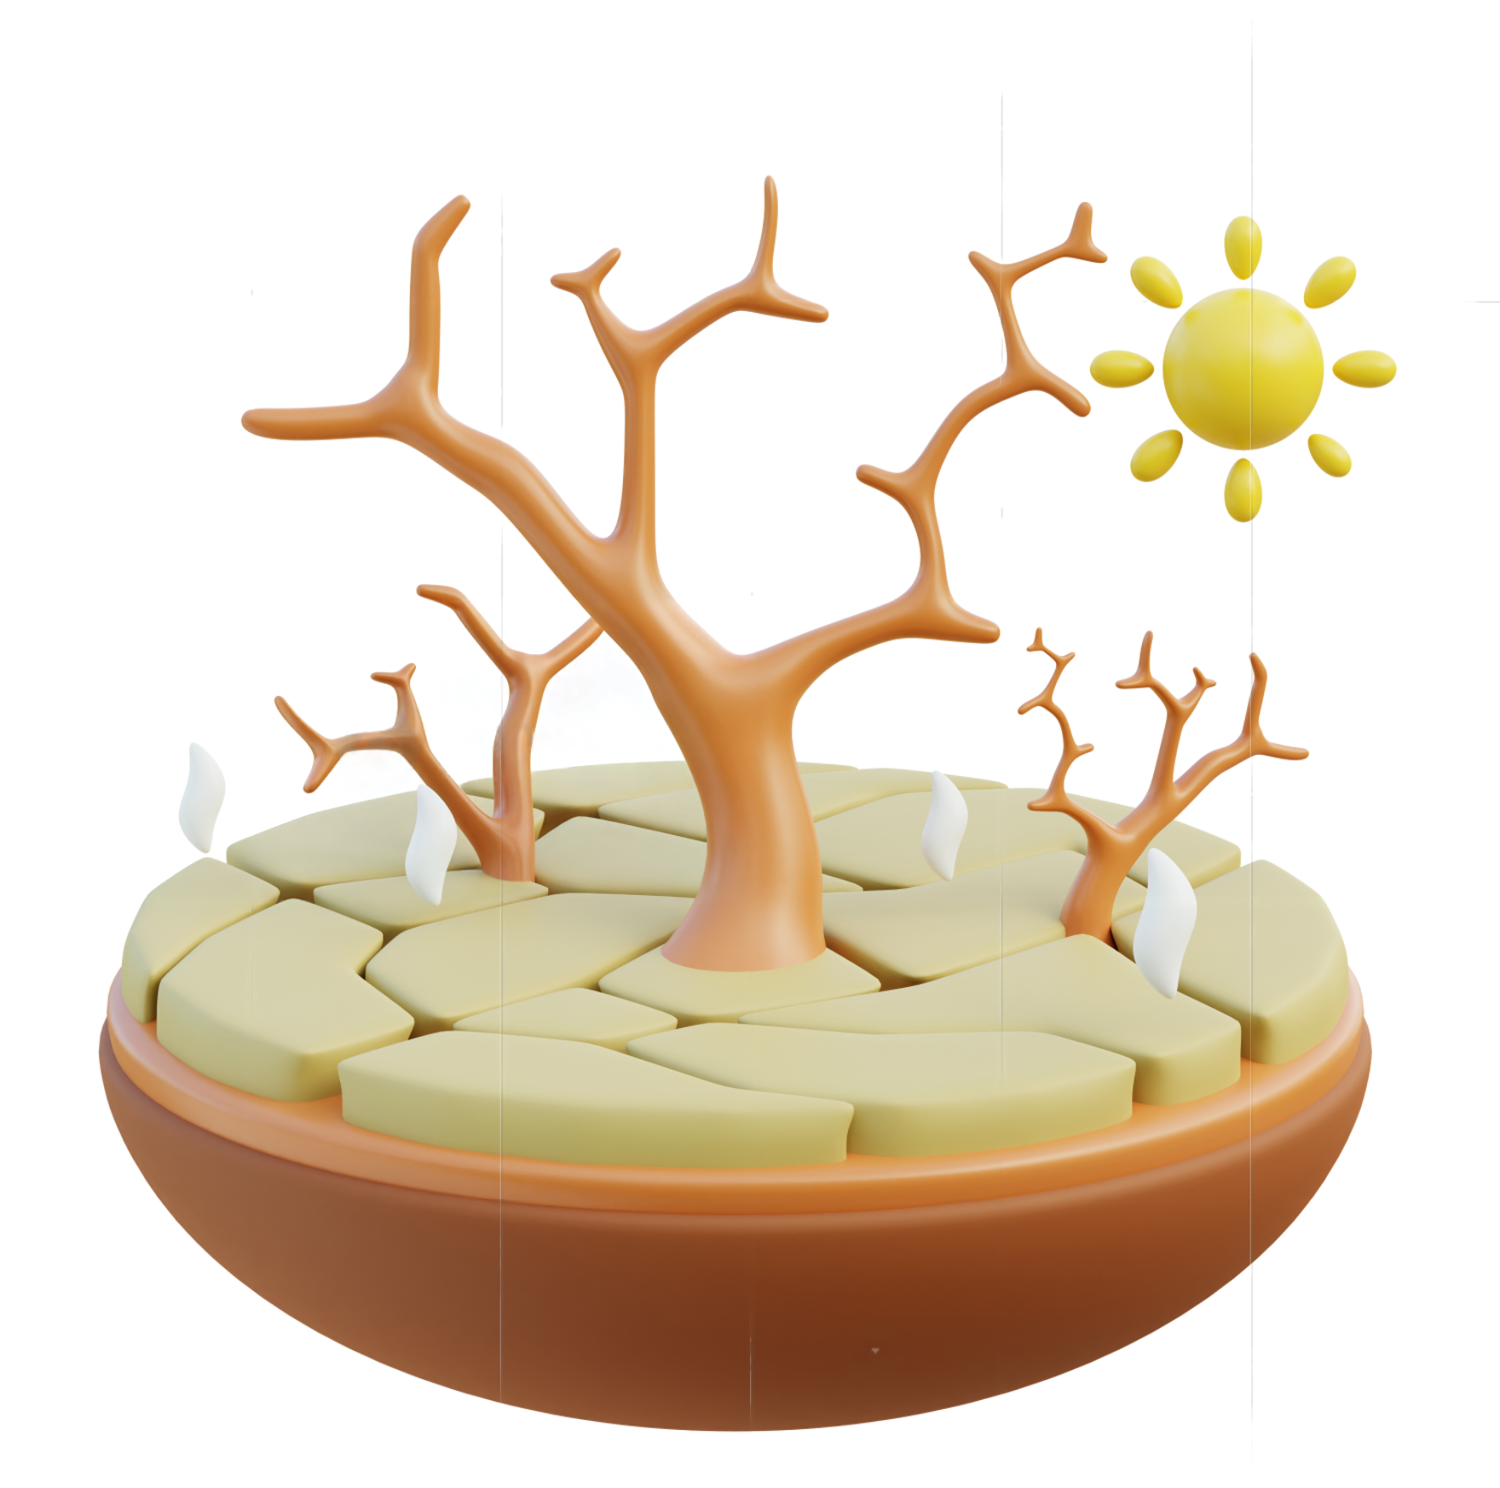
\includegraphics[height=3.4cm]{drought_cropped.png}};

                % Arrow
                \node[anchor=center] (arrow) at (2.08, 1.5)
                    {
\includegraphics[height=0.7cm]{arrow_cropped.png}};

                % Flood
                \node[anchor=south] (flood) at (4.4, 0)
                    {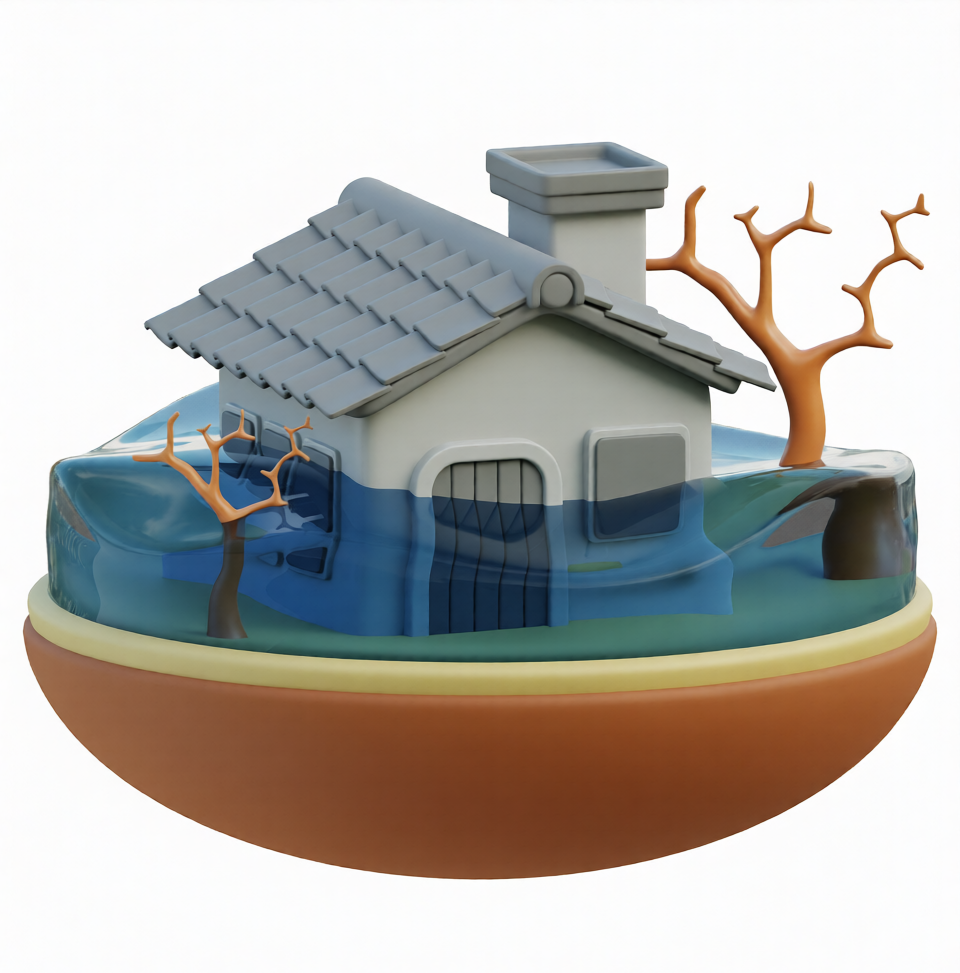
\includegraphics[height=3.4cm]{flood.png}};

            \end{tikzpicture}
        \end{column}

        % ── Right: Vertical pipeline ──────────────────────────
        \begin{column}{0.33\textwidth}
            \centering
            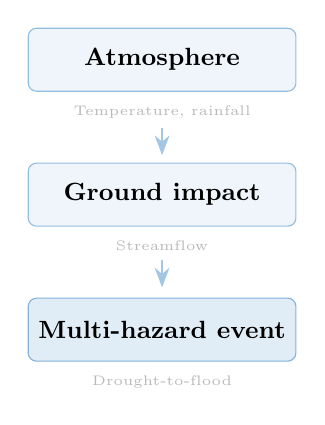
\begin{tikzpicture}[
                pipebox/.style={draw=lightblue!70, fill=lightblue!10,
                    rounded corners=3pt, minimum width=3.4cm,
                    minimum height=0.8cm, align=center,
                    font=\small\bfseries},
                sublbl/.style={font=\tiny, text=gray!55},
                arr/.style={-{Stealth[length=2.5mm]}, thick, lightblue!60}
            ]

                \node[pipebox] (s1) at (0, 0) {Atmosphere};
                \node[sublbl, below=0.05cm of s1] (l1) {Temperature, rainfall};

                \draw[arr] (l1.south) -- ++(0, -0.35);

                \node[pipebox, below=0.9cm of s1] (s2) {Ground impact};
                \node[sublbl, below=0.05cm of s2] (l2) {Streamflow};

                \draw[arr] (l2.south) -- ++(0, -0.35);

                \node[pipebox, fill=lightblue!20, draw=lightblue!80,
                      below=0.9cm of s2] (s3) {Multi-hazard event};
                \node[sublbl, below=0.05cm of s3] (l3) {Drought-to-flood};

            \end{tikzpicture}
        \end{column}

    \end{columns}

\end{frame}

\end{document}
